\documentclass[10pt,presentation]{beamer}
\usepackage[utf8x]{inputenc}
\usepackage[spanish]{babel}
\usepackage{multirow}

\mode<beamer>{%
\usetheme[hideothersubsections,
right,width=22mm]{Goettingen}
}
\title{Detecci\'on de Rasgos en la Identificaci\'on de Letras Utilizando Bubbles}
\subtitle{Intr. a Neurociencia Cognitiva y Computacional}
\author[Cossio Mercado, Gomez Mayol, Martinez Soler]{Christian Cossio Mercado, Mail\'en G\'omez Mayol, Miguel Mart\'inez Soler}
\institute{Departamento de Computación - FCEyN, UBA}
%\titlegraphic{\includegraphics[width=20mm]{USTL}}
\date{24 de Mayo de 2011}

\begin{document}

\begin{frame}%<handout:0>
  \titlepage
\end{frame}

\section{Introducci\'on}
\subsection{Revisi\'on Bibliogr\'afica}
\begin{frame}
  \frametitle{Revisión bibliográfica}
  \begin{itemize}
    \item Los papers en los que basamos nuestra investigaci\'on \ldots \pause
    \begin{itemize}
      \item Feature Detection and Letter Identification (Pelli et al., 2006) \pause
      \item Bubbles (Gosselin & Schyns) \pause
      \item Feature for Identification of Uppercase and Lowercase Letters (Fiset et al., 2008)
    \end{itemize}
\end{itemize}
\end{frame}

\subsection{Experimento}
\begin{frame}
  \frametitle{Objetivos del experimento}
  \begin{itemize}
    \item Identificar rasgos utilizados por una persona para reconocer letras de distintas tipograf\'ias  \ldots \pause
    \begin{itemize}
      \item El uso de tipograf\'ias ampliamente conocidas facilita el reconocimiento de letras \pause
      \item La eficiencia en el reconocimiento de las letras es inversamente proporcional a su complejidad \pause
      \item Los rasgos de cada letra var\'ian de acuerdo a la tipograf\'ia que se est\'e utilizando \pause
      \item Un observador ideal utilizar\'a rasgos distintos a los que utiliza una persona para identificar letras	
    \end{itemize}
\end{itemize}
\end{frame}

\begin{frame}
  \frametitle{Elecci\'on de Tipograf\'ias}
    \begin{figure}
    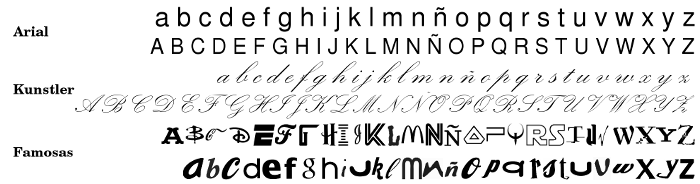
\includegraphics[scale=0.35]{graficos/letras.png}
      \caption{Conjunto completo de letras utilizadas en el experimento}
      \label{figura:conjuntoLetras}
    \end{figure}
\end{frame}

\begin{frame}
  \frametitle{Preparaci\'on de los est\'imulos}
    \begin{figure}
    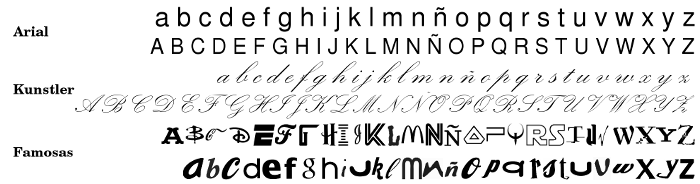
\includegraphics[scale=0.35]{graficos/letras.png}
      \caption{Preparación del estímulo final}
      \label{figura:FISET1}
    \end{figure}
\end{frame}


\section{Results}
\begin{frame}
  \frametitle{Results}
%\begin{table}[htb]
%   \tiny
%   \centering
%  \caption{PCCs for predicted vs. real binding in Fake and True methods with 2, 7 and 10 hidden neurons (best method in italics and best PCC in bold) }
%\label{tab:results}
%  \begin{tabular}{l|r||r|r||r|r||r|r}
%    \hline
%      \textbf{Allele} & \textbf{Size} & \textbf{True 02N} & \textbf{Fake 02N} & \textbf{True 07N} & \textbf{Fake 07N} & \textbf{True 10N} & \textbf{Fake 10N} \\\hline \hline
%      HLA A*0201\_09 & 3089 & \textit{0.90867} & 0.87659 & \textit{0.91133} & 0.87317 & \textbf{0.91525} & 0.87312 \\\hline
%      HLA A*0301\_09 & 2094 & \textit{0.87158} & 0.81958 & \textbf{0.88373} & 0.82268 & \textit{0.87994} & 0.82019 \\\hline
%      HLA A*3101\_09 & 1869 & \textit{0.87277} & 0.81137 & \textit{0.88504} & 0.81500 & \textbf{0.88748} & 0.81351 \\\hline
%      HLA A*0202\_09 & 1447 & \textit{0.86403} & 0.79526 & \textit{0.88985} & 0.79790 & \textbf{0.89163} & 0.80160 \\\hline
%      HLA B*5801\_09 &  988 & \textbf{0.95187} & 0.86461 & \textit{0.95122} & 0.86256 & \textit{0.94953} & 0.86070 \\\hline
%      Mamu A*01\_09  &  525 & \textit{0.90083} & 0.73711 & \textbf{0.90762} & 0.74464 & \textit{0.90414} & 0.74868 \\\hline
%      HLA A*2403\_09 &  254 & \textit{0.96759} & 0.77899 & \textit{0.96857} & 0.76313 & \textbf{0.96915} & 0.76038 \\\hline
%      HLA B*5701\_09 &   59 & \textbf{0.95035} & 0.76323 & \textit{0.94776} & 0.76913 & \textit{0.94781} & 0.77509 \\\hline
%   \end{tabular}
%\end{table}

\end{frame}


\section{Resumen}
\begin{frame}
  \frametitle{Resumen}
  \begin{itemize}
    \item \pause Para obtener Síntesis de Habla expresiva se debe tener en cuenta la situación de diálogo completa \pause
    \begin{itemize}
      \item Intenciones \pause
      \item Características de hablante/oyente \pause
      \item Relación con el oyente \pause
      \item Progreso del diálogo y nivel de entendimiento \pause
    \end{itemize}
    \item Cada técnica tiene distintas opciones para controlar la expresividad \pause
    \item Se debe regular la naturalidad obtenida vs. el control sobre lo sintetizado \pause
    \item La síntesis basada en HMM puede mejorar las limitaciones de la Selección de Unidades (datos, flexibilidad) \pause
    \item La incorporación de expresiones y contenido no-verbal puede sumar a la expresividad, pero no debe utilizarse en exceso \pause
    \item El aprendizaje automático de reglas presenta una oportunidad (e.g. para sínt. por formantes, articulación)
  \end{itemize}
\end{frame}


\end{document}
